% LC 振荡电路
% 电路|振荡电路|电容|电感

电路中电压和电流的周期性变化称为\textbf{电磁振荡(electromagnetic oscillation)} , 电磁振荡与机械振动有类似的运动形式.产生电磁振荡的电路称为振荡电路.最简单的振荡电路是由一个电容器与一个自感线圈串联而成的,称为\textbf{ LC 电路(LC circuit)}.
\begin{figure}[ht]
\centering
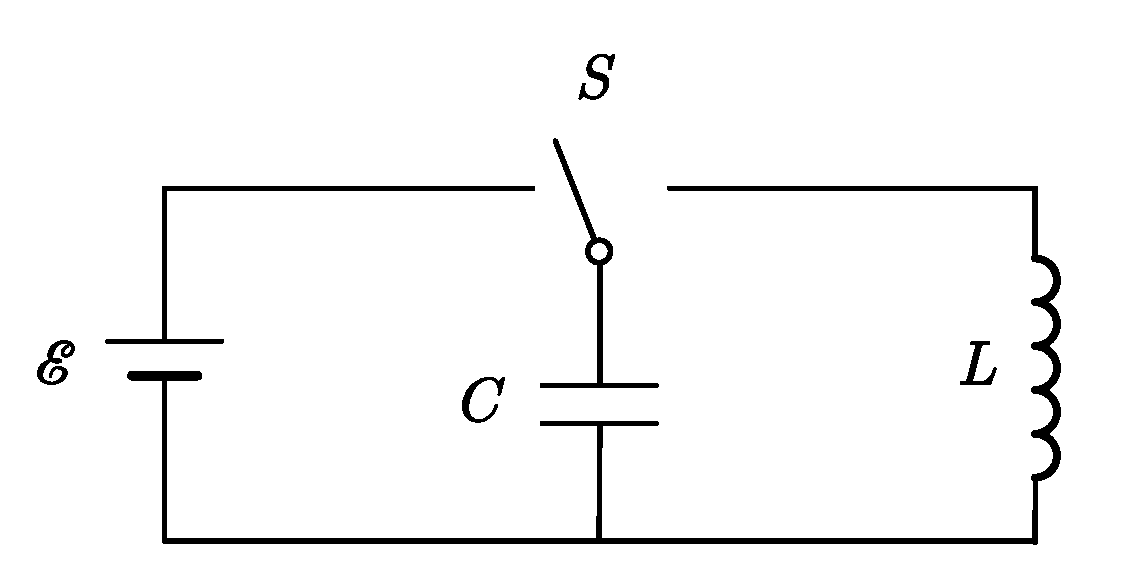
\includegraphics[width=8cm]{./figures/LC_1.pdf}
\caption{LC 振荡电路} \label{LC_fig1}
\end{figure}

如\autoref{LC_fig1} 所示的电路,先使电源给电容器充电,然后将电键接通 LC 回路,在振荡电路刚被接通的瞬间,电容器两极板上的电荷最多,板间的电场也最强,电场的能量全部集中在电容器的两极板间.

当电容器放电时,因自感的存在,电路中的电流将逐渐增大到最大值,两极板上的电荷也相应地逐渐减小到零.在此过程中,电流在自感线圈中激起磁场,到放电结束时,电容器两极板间的电场能量全部转化成线圈中的磁场能量.在电容器放电完毕时,电路中的电流达到最大值.这时,就要对电容器作反方向的充电.由于线圈的自感作用,随着电流的逐渐减弱到零,电容器两极板上的电荷又相应地逐渐增加到最大值.同时,磁场能量又全部转化成电场能量.

然后,电容器又通过线圈放电,电路中的电流逐渐增大,不过这时电流的方向与前放电时相反,电场能量又转化成磁场能量.此后,电容器又被充电,回复到原状态,完成了一个完全的振荡过程.

由上述可知,在 LC 电路中,电荷和电流都随时间做周期性的变化,相应地电容器中的电场强度和线圈中的磁感应强度以及电场能量和磁场能量也都随时间作周期性变化,而且不断地相互转化着.如果电路中没有任何能量损耗(如电阻的焦耳热、电磁辐射等),那么这种变化将在电路中一直持续下去,这种电磁振荡称为\textbf{无阻尼自由振荡}.

下面我们定量地研究无阻尼自由振荡,找出电容器极板上的电荷和电路中的电流随时间变化的规律.

设在某一时刻,电容器极板上的电荷量为$q$, 电路中的电流为$i$,并取 LC 回
路的顺时针方向为电流的正方向.线圈两端的电势差应和电容器两极板之间的电势差相等,即
\begin{equation}
-L \frac{\mathrm{d} i}{\mathrm{d} t}=\frac{q}{C}
\end{equation}
由电流的定义式$i=\dfrac{\mathrm{d} q}{\mathrm{d} t}$,我们有:
\begin{equation}
\frac{\mathrm{d}^{2} q}{\mathrm{d} t^{2}}=-\frac{1}{L C} q
\end{equation}
令$\omega^{2}=\dfrac{1}{L C}$,得
\begin{equation}
\frac{\mathrm{d}^{2} q}{\mathrm{d} t^{2}}=-\omega^{2} q
\end{equation}
根据二阶线性常系数齐次微分方程\upref{Ode2}的第3种情况,其通解为
\begin{equation} \label{LC_eq1}
q=Q_{0} \cos \left(\omega t+\phi_{0}\right)
\end{equation}
式中$Q_0$为极板上电荷量的最大值,称为电荷量振幅.$\phi_0$是振荡的初相位,$Q_0$和$\phi_0$的数值由初始条件决定.$\omega$是振荡的角频率.无阻尼自由振荡的频率和周期分别为
\begin{equation}
\nu=\frac{\omega}{2 \pi}=\frac{1}{2 \pi \sqrt{L C}}, \quad T=2 \pi \sqrt{L C}
\end{equation}

相比电荷量的变化情况,我们更关注的是电流的变化情况.由电流的定义式,对\autoref{LC_eq1} 两边求导数,得到
\begin{equation}
i=\frac{\mathrm{d} q}{\mathrm{d} t}=-\omega Q_{0} \sin \left(\omega t+\phi_{0}\right)
\end{equation}
即为电路中任一时刻的电流.

令$\omega Q_0=I_0$表示电流的最大值,称为\textbf{电流振幅},则上式为
\begin{equation} \label{LC_eq2}
i=-I_{0} \sin \left(\omega t+\phi_{0}\right)=I_{0} \cos \left(\omega t+\phi_{0}+\frac{\pi}{2}\right)
\end{equation}

\autoref{LC_eq1} 和\autoref{LC_eq2} 表明,在LC 振荡电路中,电荷和电流都作谐振动,且振荡频率相同,电流的相位比电荷的相位超前$\pi/2$.如\autoref{LC_fig2} 所示.

\begin{figure}[ht]
\centering
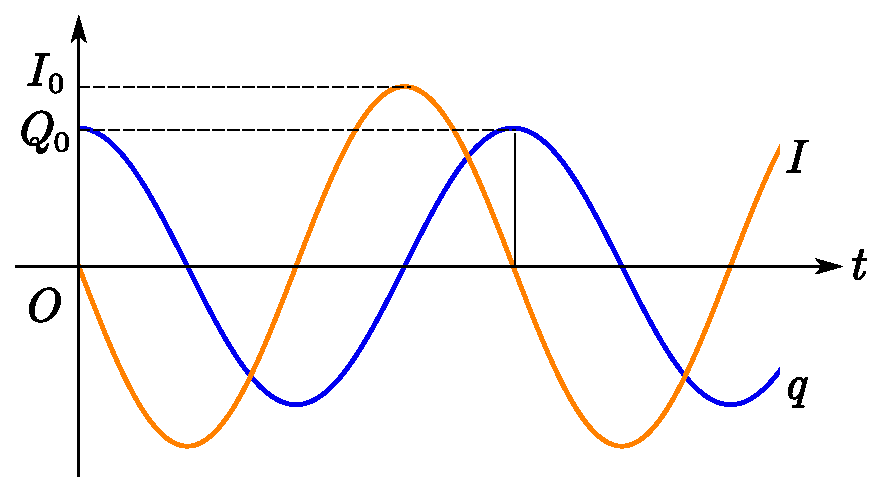
\includegraphics[width=9cm]{./figures/LC_2.pdf}
\caption{电荷与电流的振荡} \label{LC_fig2}
\end{figure}

现在让我们来考虑LC 振荡电路中的能量.在任一时刻$t$,电容器极板上的电荷量为$q$,相应的电场能量为
\begin{equation}
W_{\mathrm e}=\frac{1}{2} \frac{q^{2}}{C}=\frac{Q_{0}^{2}}{2 C} \cos ^{2}\left(\omega t+\phi_{0}\right)
\end{equation}
设此时的电流为$i$,那么线圈内的磁场能量为
\begin{equation}
W_{\mathrm{m}}=\frac{1}{2} L i^{2}=\frac{L \omega^{2} Q_{0}^{2}}{2} \sin ^{2}\left(\omega t+\phi_{0}\right)
\end{equation}
把上两式相加,并由$\omega^{2}=\dfrac{1}{L C}$,可得总能量:
\begin{equation} \label{LC_eq3}
W=W_{\mathrm{e}}+W_{\mathrm{m}}=\frac{Q_{0}^{2}}{2 C} \cos ^{2}\left(\omega t+\phi_{0}\right)+\frac{Q_{0}^{2}}{2 C} \sin ^{2}\left(\omega t+\phi_{0}\right)=\frac{Q_{0}^{2}}{2 C}
\end{equation}

\autoref{LC_eq3} 说明,在无阻尼自由振荡电路中, 尽管电能和磁能都随时间而变化,但总的电磁能量却保持不变.

从上面的分析可以知道,电磁振荡中的电荷量及电流对应机械振动中的位移和速度,自感对应于惯性,起着电流惯性作用磁场能藉对应于动能,电场能量对应于势能.在力电类比中,我们将对机械振动和电磁振荡之间的等效关系做一个完整的总结.

%电容公式
%\begin{equation}\label{LC_eq1}
%I = C \dv{U_c}{t}
%\end{equation}
%电感公式
%\begin{equation}\label{LC_eq2}
%U_L = L \dv{I}{t}
%\end{equation}
%由回路电压合为零,得
%\begin{equation}\label{LC_eq3}
%U_L + U_c = 0
%\end{equation}
%对\autoref{LC_eq1} 求导得 $\dv*{I}{t} = C \dv*[2]{U_c}{t}$, 代入%\autoref{LC_eq2} 得 $U_L = LC \dv*[2]{U_c}{t}$. 代入  \autoref%{LC_eq3}  得关于 $U_c$ 的微分方程
%\begin{equation}
%\dv[2]{U_c}{t} + \frac{1}{LC} U_c = 0
%\end{equation}
%根据二阶线性常系数齐次微分方程\upref{Ode2}的第3种情况,其通解为
%\begin{equation}
%U_c = U_0 \sin(\omega t + \phi_0) \qquad
%\omega  = \frac{1}{\sqrt {LC}}
%\end{equation}
%\begin{equation}
%I = C \dv{U_c}{t} = \sqrt{\frac{C}{L}} U_0 \cos(\omega t + \phi_0)
%\end{equation}
 
